%
% sir.tex
%
% (c) 2020 Prof Dr Andreas Müller, Hochschule Rapperswil
%
\begin{frame}
\definecolor{darkgreen}{rgb}{0,0.6,0}
\frametitle{SIR-Modell}
\vspace{-5pt}
\begin{block}{Infektionskrankheiten}
\begin{center}
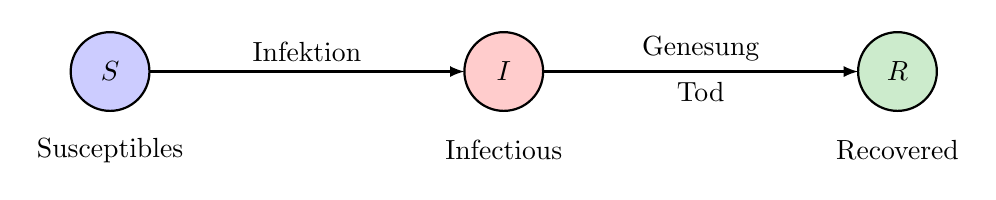
\begin{tikzpicture}[>=latex,thick]
\coordinate (S) at (-5,0);
\coordinate (I) at (0,0);
\coordinate (R) at (5,0);
\fill[color=blue!20] (S) circle[radius=0.5];
\fill[color=red!20] (I) circle[radius=0.5];
\fill[color=darkgreen!20] (R) circle[radius=0.5];
\draw (S) circle[radius=0.5];
\draw (I) circle[radius=0.5];
\draw (R) circle[radius=0.5];
\draw[->,shorten >= 0.5cm,shorten <= 0.5cm] (S) -- (I);
\draw[->,shorten >= 0.5cm,shorten <= 0.5cm] (I) -- (R);
\node at (-2.5,0) [above] {Infektion};
\node at (2.5,0) [above] {Genesung};
\node at (2.5,0) [below] {Tod};
\node at (-5,0) {$S$};
\node at ( 0,0) {$I$};
\node at ( 5,0) {$R$};
\node at (-5,-1) {Susceptibles};
\node at ( 0,-1) {Infectious};
\node at ( 5,-1) {Recovered};
\end{tikzpicture}
\end{center}
\end{block}
\vspace{-5pt}
\uncover<2->{%
\begin{block}{Differentialgleichung}
\[
\left.
\begin{aligned}
\frac{dS}{dt} &=          - \beta \, SI      \\
\frac{dI}{dt} &= \phantom{-}\beta \, SI - \gamma I \\
\frac{dR}{dt} &= \phantom{- \beta \, SI}+ \gamma I 
\end{aligned}
\quad
\uncover<3->{%
\right\}
\quad
\Rightarrow
\quad
\frac{d}{dt} (S+I+R) = 0
\Rightarrow
S+I+R=\text{const}}
\]
\end{block}}
\end{frame}
